\documentclass[sigconf,review,anonymous]{acmart}

\usepackage{booktabs}
\usepackage{listings}
\lstset{basicstyle=\ttfamily\footnotesize,breaklines=true,columns=fullflexible}

% Anonymized-artifact placeholder. Replace with anonymous.4open.science links before submission.
\newcommand{\anonurl}[1]{[link anonymized for review]}

\copyrightyear{2026}
\acmYear{2026}
\setcopyright{acmlicensed}
\acmConference[AgenticDev '26]{1st International Workshop on Agentic Software Development}{October 12, 2026}{Munich, Germany}
\acmBooktitle{Proceedings of the 1st International Workshop on Agentic Software Development (AgenticDev '26)}
\acmPrice{}
\acmDOI{}
\acmISBN{}

\begin{document}

\title{The Hypothesis Graph: A Verifiable Semantic Memory for Coding Agents}

\author{Anonymous Author(s)}
\affiliation{\institution{Anonymous Institution}\city{}\country{}}

\begin{abstract}
The \emph{hypothesis graph} is a data structure for coding agents that deepens their reasoning and makes them accountable. Implemented at the harness layer, its nodes are testable claims, its edges the refutations that name the next claim. It updates by inquiry, Peirce's typed loop of abduction, deduction, and induction. What is new is running that loop as mechanical harness operations around the one step no procedure reaches. That step, the abductive leap, stays in the model; the harness manufactures the surprise, fires the kill, and records the trail, instead of leaving the loop to a model's undifferentiated prose. We demonstrate the mechanism on one contamination-free bugfix. Six self-attested arms plateau at a narrow fix; an externally verified comparator, the one input a context-bound agent cannot author for itself, carries a weaker model (Sonnet 4.6) to the behavior of the merged human fix that the strongest released model (Fable 5) does not reach without it. This buys verifiable accountability and reasoning that persists past the context window, at no additional training cost, usable by any coding-agent harness that can run pinned trials and read their verdicts.
\end{abstract}

\begin{CCSXML}
<ccs2012>
<concept>
<concept_id>10011007.10011074.10011099</concept_id>
<concept_desc>Software and its engineering~Software verification and validation</concept_desc>
<concept_significance>500</concept_significance>
</concept>
<concept>
<concept_id>10010147.10010178</concept_id>
<concept_desc>Computing methodologies~Artificial intelligence</concept_desc>
<concept_significance>300</concept_significance>
</concept>
</ccs2012>
\end{CCSXML}
\ccsdesc[500]{Software and its engineering~Software verification and validation}
\ccsdesc[300]{Computing methodologies~Artificial intelligence}

\keywords{hypothesis graph, agent memory, abductive inference, LLM agents, provenance, auditability, falsifiability, post-cutoff evaluation}

\maketitle

\section{Introduction}\label{sec:intro}

In coding agents, the LLM is wrapped in a harness: the verification, testing, and memory a software task needs. The field building these is moving up a level of abstraction, from the model to the harness. Roychoudhury et al.~\cite{roychoudhury2025} reframe the goal as \emph{programming with trust}, arguing that deployment turns on verification, testing, and analysis built into the agent rather than on raw generation. Liu et al.~\cite{liu2024survey} survey agents for software engineering and organize the field around those same missing pieces; Yehudai et al.~\cite{yehudai2025} add that scoring final outputs misses the reasoning and failure causes inside a run, and call for trajectory-level assessment; Wang et al.~\cite{wang2025survey} list persistent, structured memory among the open challenges.

A patch passes the visible tests, but that's not enough: passing certifies only the cases the tests cover. An over-narrow patch passes them and is wrong off-suite. Confirming it means reconstructing the reasoning the agent never recorded, at a cost approaching that of producing it, so the work shifts from writing to checking. Code review is the bottleneck.

When reasoning is discarded, each run rebuilds context from scratch. Even where agent memory adopts the cognitive-architecture lineage, as CoALA~\cite{coala} does in mapping it onto Soar~\cite{soar} and ACT-R, the semantic slot stores facts rather than a falsifiable structure, so the search is discarded once a patch passes. At best, a trail of blobs is saved as provenance.

Here we give the agent a trail of verifiable knowledge. The \textbf{hypothesis graph} is a semantic memory that holds an agent's reasoning while it works. The fix arrives with the inquiry that produced it: what was hypothesized, what was tested, what was ruled out. Each step carries a trial a stranger can rerun. The promise reverses the trust assumption by shifting the burden of proof outside the agent. The model still reasons, but each node it produces is checkable on its own at the harness layer, independent of the model.

Two contributions run through this, and they are separable. The graph is the accountability substrate, and its value is argued by construction: every node replays. The externalized comparator is the capability mechanism, and its value is shown by ablation. The graph makes reasoning checkable; the comparator supplies the one verdict a self-graded agent cannot author for itself. Keeping them apart is what lets the ablation below read cleanly, where several arms share the graph and only the verdict source moves.

What that buys is not incremental. On one contamination-free bug, an externalized comparator carried a weaker model to a fix the strongest released model could not reach without it (\S\ref{sec:case}): a capability lift, where a scaffold usually buys only automation.

\section{The Hypothesis Graph}\label{sec:graph}

\subsection{Requirements}

A semantic memory that holds an agent's live reasoning must clear four requirements at once. \emph{Holds hypotheses}: stores a hypothesis still under consideration, where prose, skill libraries, and retrieval keep only verified facts and established chunks. \emph{Refutable by test}: each claim carries a kill condition, the executable test that can prove it wrong. \emph{Independently verifiable}: a stranger verifies a conclusion by rerunning its recorded trial, instead of re-deriving the reasoning or taking the author's word. \emph{Persistent}: the trail persists past the context window rather than being discarded once a patch passes. Table~\ref{tab:structures} places prior structures against these requirements.

\begin{table}
\caption{Prior structures against the four requirements ($\bullet$ native, $\circ$ with common extensions, --- needs another layer).}
\label{tab:structures}
\small
\begin{tabular}{lcccc}
\toprule
Structure & Hyp. & Tests & Indep.\ verif. & Persist. \\
\midrule
\textbf{Hypothesis graph} & $\bullet$ & $\bullet$ & $\bullet$ & $\bullet$ \\
Truth-maintenance~\cite{doyle1979,dekleer1986} & $\bullet$ & $\circ$ & $\circ$ & $\circ$ \\
Provenance (W3C PROV~\cite{prov}) & $\circ$ & $\circ$ & $\circ$ & $\bullet$ \\
Search/proof tree~\cite{cegar,cegis} & $\bullet$ & $\circ$ & $\circ$ & $\circ$ \\
Argumentation~\cite{dung1995} & $\bullet$ & $\circ$ & $\circ$ & $\circ$ \\
ReAct trace~\cite{react} & $\bullet$ & $\circ$ & $\circ$ & $\bullet$ \\
\bottomrule
\end{tabular}
\end{table}

An LLM is what finally fills the gap. Filling the graph takes a reasoner that reads a surprising failure, proposes candidate causes in open vocabulary, and turns each into an executable test, with no hand-built domain model. Classical inference engines could do this only inside a formalism encoded by hand, which is why the slot stayed a research program; the LLM populates it across arbitrary codebases, which is what makes the structure practical here.

\subsection{Graph semantics}

The structure meets all four requirements with three pieces: a node, an edge, and one invariant. A \textbf{node} is a claim bound to a trial: a hypothesis, the perturbation that tests it stated as an exact command, the observed outcome, and a credence typed by the reasoning mode that established it. An \textbf{edge} is generated by a kill condition: the manner of a hypothesis's death names the next hypothesis, so the structure is self-extending, with no external controller deciding where to look.

\begin{quote}
\textbf{Replay invariant.} Every node is reconstructible, by a stranger who does not trust the author, from its recorded trial alone: the exact command, the observed outcome, the verdict, and the credence cap.
\end{quote}

The contract holds on the node's mechanical skeleton; the hypothesis prose the node also carries falls outside it, by design. The prose is the part an auditor would otherwise have to trust, and the recorded trial is what replaces trusting it, so the invariant draws its line exactly where checkability begins.

Five operations maintain the structure, each defined with a one-clause argument that it preserves the invariant. \emph{Create} appends a node; a node is admitted only if its trial replays, so the invariant holds by induction over reachable graphs. \emph{Read/replay} reconstructs any node by re-running its recorded trial. \emph{Classify} marks a node \emph{killed} or \emph{witnessed} on its trial's outcome and caps its credence at the mode that earned it; it appends a verdict and never edits the recorded trial. \emph{Link} is the one genuinely novel operation: the manner of a hypothesis's death names the next hypothesis, so a classification spawns the next node with no external controller. \emph{Prune} removes a dead branch from the working frontier while its record stays in place, so every pruned node replays exactly as before.

\begin{figure}
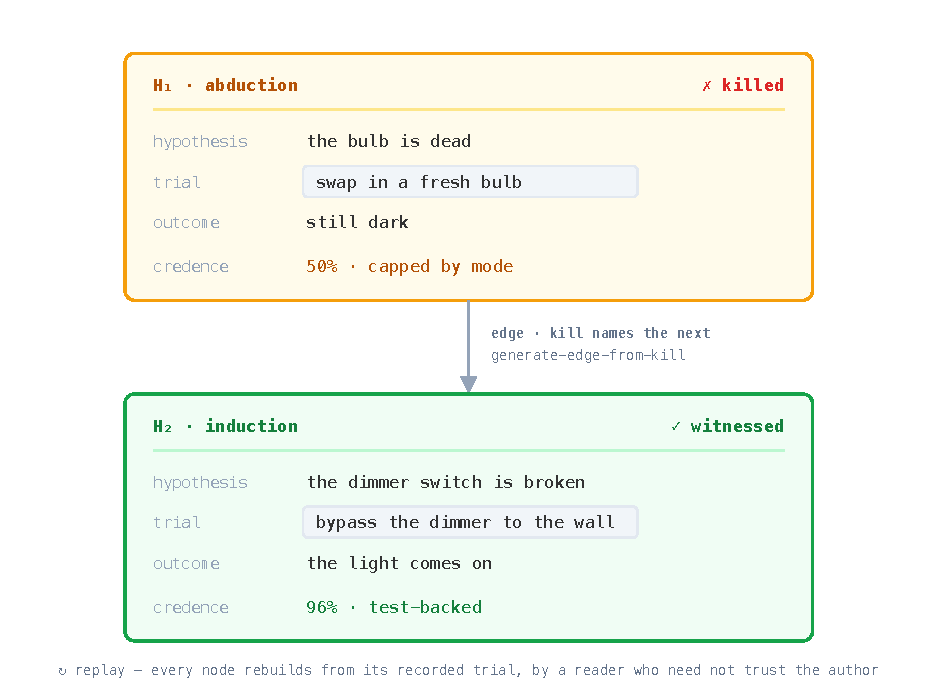
\includegraphics[width=\linewidth]{hypothesis-graph-anatomy.pdf}
\caption{Two nodes and the edge between them on a dead-light inquiry. The bulb hypothesis is killed by a cheap trial; its death names the next node, the dimmer, which a second trial witnesses. Each node binds a hypothesis to a trial, an observed outcome, and a credence capped by the mode that earned it. Every node rebuilds from its recorded trial, so an auditor replays the structure instead of trusting it.}
\label{fig:anatomy}
\end{figure}

\subsection{Auditability}

The invariant yields a property no benchmark can evaluate:

\begin{quote}
\textbf{Local replay auditability.} Any single conclusion is checkable by re-running that node's one recorded trial, without reconstructing the inquiry and without extending trust to whoever ran it.
\end{quote}

This is, for inquiry, the analogue of a certificate a consumer checks without trusting the producer, and like the Merkle audit path or proof-carrying code~\cite{necula1997}, its value rests on a contract; a complexity bound is beside the point. Two grades matter. Where the trial is a deterministic command over pinned inputs, replay is \emph{strong}: re-execution reproduces the recorded outcome, and the lead case (\S\ref{sec:case}) is here. Where the trial runs a model or a live service, replay is \emph{artifact-level}: the recorded output is verified and the deterministic predicate re-run over it.

The nodes are ordinary; what is novel is the edge semantics. A search tree finds; a proof tree justifies. The hypothesis graph is both at once, because the search path \emph{is} the justification: every step was a trial. Refinement is the closest kin: in CEGAR~\cite{cegar} and CEGIS~\cite{cegis} a counterexample \emph{is} a kill that names the next experiment. What is novel is running that loop over an \emph{open} hypothesis space abduced in domain vocabulary. Replayability stands in for the sound abstraction a closed setting supplies for free, with completeness as the price the open move forfeits. Truth-maintenance systems~\cite{doyle1979,dekleer1986} maintain belief status under assumptions, but the empirical trial and the kill-generated successor are external conventions; provenance~\cite{prov} records replayable activities yet does not decide which hypothesis comes next; a ReAct trace~\cite{react} is an append-only log whose continuation policy the controller decides and the record never holds. What the hypothesis graph adds is their composition in one append-only object: an open-domain hypothesis, its executable trial, its kill condition, and the successor that kill names.

\section{Methodeutic Grounding}\label{sec:method-grounding}

A store of causal knowledge needs reasoning to be encoded into it. The insight, the leap to a candidate cause, stays with the model, but the harness needs a method to stage reasoning. Peirce~\cite{peirce1878,peirce1903} types the operations of inquiry into three irreducible modes: \emph{abduction} generates explanatory hypotheses for surprising observations; \emph{deduction} derives testable predictions from hypotheses; \emph{induction} tests predictions against evidence. No single mode carries a belief to its grade: abduction proposes content but does not test it; induction tests but introduces no new explanatory content; deduction traces consequences but invents nothing.

Collapse the modes and you get familiar failure modes: confirmation bias (induction without abductive alternatives), confabulation (abduction without inductive grounding), free-association (no typed mode at all). That collapse is exactly what modern LLM agents do by default, since a single forward pass proposes, predicts, evaluates, and rationalizes in undifferentiated prose.

The surprise has a primitive, and it is a diff: a before snapshot, an after snapshot, and the perturbation that flipped, read as figure against the ground that held. Separation logic calls the frame-inference half of this \emph{bi-abduction} and scaled it in Facebook Infer~\cite{biabduction}; it localizes where belief and code diverge and leaves the leap to what would explain it unmade. Debugging automation has run some version of this loop for decades: spectrum-based fault localization~\cite{jones2002}, delta debugging~\cite{zeller2002}, model-based diagnosis~\cite{reiter1987}, search-based repair~\cite{legoues2012,monperrus2018}. Those tools automate the loop; what is new is that the hypothesis graph \emph{persists} it as a typed, replayable structure, and that an LLM abduces the hypothesis space open-vocabulary rather than inside a hand-built domain model. The difference from a Bayesian network~\cite{pearl1988} runs deeper than dropped probabilities: a Bayes net conditions over a fixed variable set it is handed; the hypothesis graph generates the space as the inquiry runs, its edges genealogical rather than conditional.

\section{The Methodeutic Harness}\label{sec:harness}

The loop that writes the graph needs four things: \emph{iteration} (one pass can't be trusted, so the loop re-enters on failure); a \emph{deterministic oracle} (a model can't be trusted to catch its own bias, so the check comes from outside the weights); \emph{three typed modes}, each capped at its own confidence; and \emph{semantic memory} (the reasoning is recorded into the hypothesis graph and survives the context window).

Concretely, this is a skill with a tool call in a loop: an outer deterministic driver invokes an agent via an \texttt{inquire} skill, which accesses a deterministic comparator tool (\S\ref{sec:abductor}). \texttt{inquire} builds the graph with each node typed by the mode that established it: abduction proposes candidate root causes and writes hypothesis nodes with falsifiable predicates and kill conditions (low confidence); deduction traces each hypothesis's consequences to localize the suspect set (high); induction tests survivors with cheap read-only experiments (moderate). \texttt{implement} then writes the surviving hypothesis, with an adversarial challenger critiquing the diff against the spec. \texttt{attest} runs the test suite, takes the grader's pass/fail verdict, and emits a re-entry route from a fixed verdict-to-route table. The driver parses the verdict and the route; both are mechanical, and no model decides termination. Kill conditions are mechanical predicates over the evidence trajectory, so a node dies when its predicate fires and not before. The graph persists across iterations; re-entry adds nodes rather than overwriting, so the graph doubles as the loop's checkpoint and no dead branch is re-proposed.

Code is the right substrate because it combines three properties other inquiry domains rarely bring together: it is \emph{reproducible} (same input yields same output, modulo controlled nondeterminism), \emph{deterministic} (causal lines from input to behavior are mechanical), and \emph{perturbable} (single-line diffs are cheap to apply and fully observable). Because those three hold together, kill conditions over code are exact executions, and a single passing test on a captured diff is a complete verdict for that case.

\section{The Mechanism by Case Study}\label{sec:case}

What would prove that we had encoded reasoning into the harness, rather than just prompted a model into a better answer? The signal has to be one prompting alone can't produce: without the reasoning operation, the bare model can't reach the fix; handed the operation, it reaches the fix; and the fix generalizes to cases it was never shown.

\subsection{Why not a benchmark}

We first went looking for that signal on an established coding benchmark, and learned such benchmarks aren't built to show it. A SWE-bench-shaped task hands the solver the issue text, the repository, and a hidden test the fix must turn green; the issue text often hands over the specification, removing the discovery step. In our determinacy audit of all 728 public SWE-bench Pro~\cite{swebenchpro} tasks (artifact: \url{https://anonymous.4open.science/r/weaudit-901E}), the well-specified majority is one-shot for a competent model, and the underdetermined floor (15.0\%) grades the author's unstated intent, undiscoverable from the materials. With the tests as oracle, our harness resolves 95.3\% of the public split under the official grader (artifact: \url{https://anonymous.4open.science/r/wepro-3D87}): an artifact of iterating against the answer key rather than a leaderboard result, and evidence that specification-to-implementation translation is largely solved. The interesting work is discovery, and the public set carries contamination risk besides. So we went looking for a post-cutoff bug where discovery is the whole difficulty.

\subsection{Verus \#2219}

The bug is verus-lang/verus\#2219: ghost uses of the never type invalidate borrow-checking. Verus is a deductive verifier for Rust; the cardinal property of any verifier is soundness, and an unsoundness, where the verifier blesses a program it owes a rejection, is the worst defect it can carry and the hardest to notice, since the symptom is silence. The issue is from March 2026, opened and fixed after the solve models' training cutoffs, so the case is contamination-free. The maintainer's narrow fix (PR \#2230) passes its shipped test; a general fix landed three months later (PR \#2501).

The correct fix must range over a whole class of inputs. A \emph{ghost} expression of type \texttt{!}, erased before compilation and so not actually diverging, still triggers rustc's never-type edge prune: Verus drops a live control-flow edge and verifies a program it owes a rejection. Two programs identical at the \texttt{!} token owe opposite verdicts, depending on whether the divergence is ghost-erased or genuine. The narrow fix keys on the surface token; the general fix keeps the edge for the whole class of uninhabited types the token never names. That distinction, the symmetric difference (XOR) between the two behaviors, is what the experiment lives on. Three further properties make it a good study: the general fix took deep Verus knowledge and three months; the symptom sits four causal steps from the fault, so localization has to climb; and the project's own suite passes for \emph{both} fixes, so it cannot see the distinction.

\subsection{Experiment design}

We hold one reproducible control and ablate two factors for attribution (Table~\ref{tab:arms}): the \emph{verification mechanism}, whether each kill gets its verdict by the model's own attestation (self-attested) or against a reference the model cannot author (externally verified); and the \emph{inquiry tier}, whether the typed loop runs in the prompt or is lifted out as a tool call. Each arm writes a hypothesis graph by the same loop and runs three times, with one preregistered sentence per loop: testing X, predict Y, refuted by Z. For ecological accuracy each model runs in its own native agent CLI (Claude models in Claude Code, GPT-5.5 in codex, Composer 2.5 in Cursor); the meta-loop owns only the stage contracts, the graph, and the gate.

\begin{table}
\caption{Ablation arms, least to most intervention ($\bullet$ present, $\circ$ absent).}
\label{tab:arms}
\small
\begin{tabular}{lccc}
\toprule
Arm & Enumeration & Kill cond. & Ext.\ verified \\
\midrule
minimal / neutral prompt & $\circ$ & $\circ$ & $\circ$ \\
site-enumeration prompt & $\bullet$ & $\circ$ & $\circ$ \\
abduction prompt & $\circ$ & $\bullet$ & $\circ$ \\
hypothesis-graph prompt & $\circ$ & $\bullet$ & $\circ$ \\
self-verifier harness & $\bullet$ & $\bullet$ & $\circ$ \\
comparator-enabled harness & $\bullet$ & $\bullet$ & $\bullet$ \\
\bottomrule
\end{tabular}
\end{table}

To score every arm on the same mechanical ruler we build a tiny answer key: three compiler states (the buggy base, the narrow fix, the general fix) plus a handful of probe programs, each owed one correct verdict, \texttt{REJECT} for unsound, \texttt{ACCEPT} for sound. Bug probes are uninhabited by construction, so their correct \texttt{REJECT} is free and the base compiler is wrong on exactly them. Divergence probes are the hard side: sound, to be preserved, and invisible to the gate's grammar; their \texttt{ACCEPT} comes from the merged human fix and stays held out. Passing them therefore tests whether a fix represents the rule rather than fits the gate. A recall probe rules out memorization: asked in isolation how \#2219 was fixed, the model does not recover the patch. Every verdict is from a forced-fresh, fingerprinted build; the frozen dataset and regrade script are committed (\url{https://anonymous.4open.science/r/hymech-117E}).

\subsection{The comparator tool}\label{sec:abductor}

The externalized comparator is released as an open-source command-line tool (\url{https://anonymous.4open.science/r/comparator-DA10}). It does three domain-general operations with no answer built in: it \emph{enumerates} a case space closed under the property's type-formers, wider than any one hypothesis; it \emph{calibrates} each case against a known-good baseline, so the ground truth is external to the model; and it \emph{gates} on a single pass/fail signal the model iterates against. The prompt demands generality and supplies the signal, so the rule is the model's own reconstruction: the comparator returns only pass/fail on candidate behavior, never the patch, the predicate, or the API.

\subsection{Results}

The six self-attested methods plateaued at the narrow fix on all eighteen draws; only the externally verified arm broke past (Table~\ref{tab:results}). Its fix flips the whole bug-set, rejects two out-of-grammar held-outs it never saw, and stays wide-but-broken exactly where the gate's grammar is silent, the divergence side. Extend the gate's coverage to the divergence case and the same fix lands across four models in four native CLIs (Fable, Sonnet 4.6, Composer 2.5 reach the general fix's behavior; codex clears the bug side but cannot implement the divergence case, an implementation limit the verdicts do not remove).

\begin{table}
\caption{Six self-attested arms vs.\ the comparator arm. Cases flipped is the modal of three draws.}
\label{tab:results}
\small
\begin{tabular}{lccl}
\toprule
Arm & Gate pass & Flipped & Outcome \\
\midrule
minimal / neutral & --- & 114 & narrow plateau \\
site-enumeration & --- & 114 & narrow plateau \\
abduction & --- & 114 & narrow plateau \\
hypothesis graph & --- & 114 & narrow plateau \\
self-verifier & --- & 114 & narrow plateau \\
comparator & \checkmark & 269 & general on bug-set \\
\bottomrule
\end{tabular}
\end{table}

The headline lift is a slice across two models: the same bug handed to the strongest released model without the comparator, and to a weaker one with it (Table~\ref{tab:lift}). Without the comparator neither matches the merged fix, and they miss in opposite directions: Fable too wide, Sonnet too narrow. With it both reach the merged fix's behavior on the committed probes. The match is reconstruction, not lookup.

\begin{table}
\caption{Two contamination-clean models, one harness, gate covering divergence. One draw per cell.}
\label{tab:lift}
\small
\begin{tabular}{lcc}
\toprule
 & No comparator & + comparator \\
\midrule
Fable 5 (strongest released) & wide-but-broken & \#2501 behavior \\
Sonnet 4.6 & narrow (\#2230) & \#2501 behavior \\
\bottomrule
\end{tabular}
\end{table}

\begin{figure}
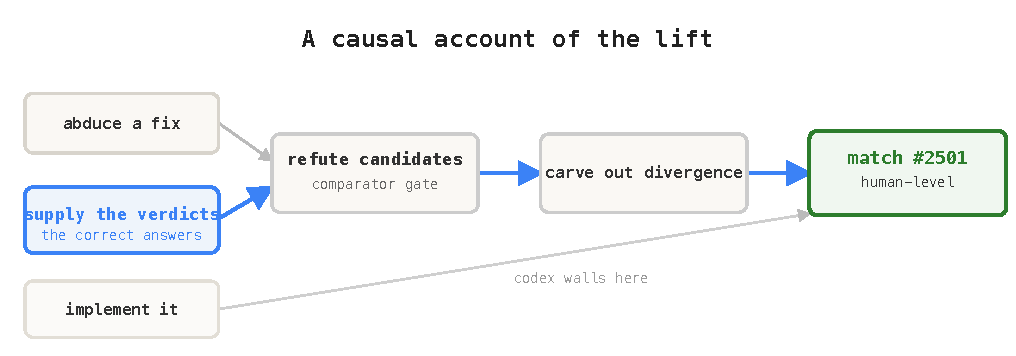
\includegraphics[width=\linewidth]{verus-2219-lift-mechanism.pdf}
\caption{The ablation as one causal diagram. Four factors stay identical across arms (model, loop, bug, graph), so none can be the cause; only the verdict source varies. Gray boxes the model can build for itself; the blue box is the one input it cannot author.}
\label{fig:mechanism}
\end{figure}

\subsection{Why the cheaper explanations fall}

\emph{Did the comparator just search harder?} The self-verifier searched exactly as hard: handed the same prompt and no tool, it built its own case generator and brute-forced some 7,026 cases a round, and still plateaued, grading against its own belief. Enumeration sat on both sides of the comparison, so it is not the lever. Nor is reasoning depth: the abduction arm ran textbook bi-abduction to the semantic predicate the general fix turns on, named it in prose, self-validated it against its own programs, and still shipped the same narrow patch as the one-line minimal arm.

\emph{Was the model handed the fix?} It was handed correct verdicts on cases. It never saw the patch, the predicate, or the Rust API; it still localizes the fault four steps up the chain and writes the fix itself.

\emph{A better scaffold, then?} The self-verifier is the scaffold control: the whole loop, enumeration and kill conditions included, with the external verdict the only piece removed. It plateaus beside the bare prompt.

\emph{Just the stronger model?} The attribution rests on the within-model contrast, where the model is held fixed and only the verdict source moves. The cross-model grid only illustrates the consequence; the within-model ablation proves the cause.

A model can bootstrap the \emph{enumeration}, because that is mechanical: handed a vague prompt and no gate, Fable rebuilt one for itself, its own 7,026-case gate over the uninhabited type-formers. It cannot bootstrap the \emph{correct verdicts}: its self-built gate labels each case with the very predicate under test, so the one case that needs a truth from outside its own belief gets self-mislabeled as handled. The claim is scoped to that self-grading circularity. Retrospectively the correct verdicts are free, mined from approved history (the merged fix, the regression suite); prospectively, on a fresh bug, the easy side has one and the hard side costs a human judgment. That division of labor is the deployment design, and nothing is hidden.

\section{Related Work}\label{sec:related}

\emph{Scaffolds and harnesses.} SWE-bench-targeted harnesses (OpenHands~\cite{openhands}, SWE-agent~\cite{sweagent}, AutoCodeRover~\cite{autocoderover}) are ReAct-pattern loops without a falsifiable memory structure. Recent results report a weaker model with a scaffold beating a stronger one on the \emph{automation} axis: GradleFixer~\cite{gradlefixer} via domain-specific Gradle primitives, Confucius Code Agent~\cite{confucius} via a whole-scaffold effect that reverses when the stronger model gets the same scaffold. The lift here differs on three counts: it is a frontier extension rather than a throughput gain; the externalized operation is domain-general, carrying no answer and no domain model; and a controlled ablation pins it to the verdict source alone, so it does not reverse when the stronger model is handed the same harness. SWT-Bench~\cite{swtbench} uses the same external-golden shape but as an evaluation oracle for test generation; ours is a runtime instrument the agent iterates against with the answer key hidden.

\emph{Typed reasoning and graph memory.} Theorem-of-Thought~\cite{tot} types reasoning into abductive/deductive/inductive agents per query: the typed cycle without a persistent typed memory. Cognitive Memory Manager~\cite{cmm} extracts a typed-node DAG by observing agent execution: the typed graph, mined descriptively where ours is generative (kills fire live and route the run). IDEA~\cite{idea} and ADI~\cite{adi} run explicitly Peircean loops in non-SE domains. FVDebug~\cite{fvdebug} builds a debugging hypothesis graph but selects the next node by asking the model, the arbiter this work removes. What the ablation adds to this cluster is which piece is decisive: not the graph structure, which several share, but where a kill edge gets its ground truth.

\emph{Benchmark validity.} SWE-Bench+~\cite{swebenchplus} found solution leakage and weak tests by manual audit; LiveCodeBench~\cite{livecodebench} originated post-cutoff evaluation. The standard objection, that cutoffs are porous, is answered here by construction: the case is post-cutoff and the solving model's weights predate the fix.

\section{Limitations}\label{sec:limits}

The mechanism evidence is existence-grade: one audited divergence, on one instance, in a program that was not preregistered when it ran. Nothing here is a rate. On pilots from a merged-PR pool, a minimal baseline solved most bugs unaided; the band where the mechanism engages is bounded below by baseline reach and above by triage, which is why a population rate over an unselected pool would measure the band's width and miss the mechanism. The loop-versus-corpus control is unrun: whether the lift comes from iterating against the gate or from the labeled cases alone has a separating control (a one-shot pass over the static cases, no loop) that has not been run. The memory is small and per-instance, one markdown file per inquiry; cross-instance accumulation is untested. The central claims are built to fail loudly: the mechanism claim dies if the committed receipt fails to replay or a discriminating program shows the externally verified fix wrong where the human fix is right; the encoding-boundary claim dies if a self-graded model reaches the hard side with labels it authored independently of the predicate under test; the attribution dies if the bracket fails to replicate from its preregistered sample.

\section{Conclusion}\label{sec:conclusion}

In the domain where every step is checkable, an agent's reasoning can be made accountable rather than merely trusted. The hypothesis graph is a replayable record that submits each generated step to a world-facing trial and retains only what survives; it reduces the cost of relying on an agent from reproducing its work to rerunning its record. Inside that checkable domain sits a bolder result: on a single contamination-free bug, the externalized comparator carried Sonnet 4.6 to a fix Fable 5 could not reach without it, a capability lift attributed by within-model ablation to the verdict source, the one input the model cannot author, with no training involved.

\subsection*{Artifact availability and LLM disclosure}
All code and data are openly available and DOI-archived; links are anonymized for review. The comparator tool, the mechanism experiment (preregistration, frozen dataset, regrade script, climb traces), the bench run, and the determinacy audit each reproduce from committed inputs. LLMs are the subject of study, an instrument, and a writing aid; claims, methodology, numbers, and argument structure are the authors'.

\begin{thebibliography}{40}

\bibitem{roychoudhury2025} A. Roychoudhury et al. 2025. AI Software Engineer: Programming with Trust. arXiv:2502.13767.
\bibitem{liu2024survey} J. Liu et al. 2024. Large Language Model-Based Agents for Software Engineering: A Survey. arXiv:2409.02977.
\bibitem{yehudai2025} A. Yehudai et al. 2025. Survey on Evaluation of LLM-based Agents. arXiv:2503.16416.
\bibitem{wang2025survey} Y. Wang et al. 2025. A Survey of AI Agent Programming Systems. arXiv:2508.11126.
\bibitem{coala} T. Sumers, S. Yao, K. Narasimhan, and T. Griffiths. 2024. Cognitive Architectures for Language Agents. TMLR. arXiv:2309.02427.
\bibitem{soar} J. Laird, A. Newell, and P. Rosenbloom. 1987. Soar: An Architecture for General Intelligence. \textit{Artificial Intelligence} 33.
\bibitem{doyle1979} J. Doyle. 1979. A Truth Maintenance System. \textit{Artificial Intelligence} 12.
\bibitem{dekleer1986} J. de Kleer. 1986. An Assumption-based Truth Maintenance System. \textit{Artificial Intelligence} 28.
\bibitem{prov} L. Moreau et al. 2013. PROV-DM: The W3C Provenance Data Model.
\bibitem{cegar} E. Clarke, O. Grumberg, S. Jha, Y. Lu, and H. Veith. 2000. Counterexample-Guided Abstraction Refinement. In \textit{CAV}.
\bibitem{cegis} A. Solar-Lezama et al. 2006. Combinatorial Sketching for Finite Programs. In \textit{ASPLOS}.
\bibitem{dung1995} P. M. Dung. 1995. On the Acceptability of Arguments. \textit{Artificial Intelligence} 77.
\bibitem{react} S. Yao et al. 2023. ReAct: Synergizing Reasoning and Acting in Language Models. In \textit{ICLR}.
\bibitem{necula1997} G. Necula. 1997. Proof-Carrying Code. In \textit{POPL}.
\bibitem{peirce1878} C. S. Peirce. 1878. Illustrations of the Logic of Science. \textit{Popular Science Monthly}.
\bibitem{peirce1903} C. S. Peirce. 1903. Pragmatism as the Logic of Abduction. Harvard Lectures on Pragmatism.
\bibitem{biabduction} C. Calcagno, D. Distefano, P. O'Hearn, and H. Yang. 2009. Compositional Shape Analysis by Means of Bi-Abduction. In \textit{POPL}.
\bibitem{jones2002} J. Jones, M. J. Harrold, and J. Stasko. 2002. Visualization of Test Information to Assist Fault Localization. In \textit{ICSE}.
\bibitem{zeller2002} A. Zeller and R. Hildebrandt. 2002. Simplifying and Isolating Failure-Inducing Input. \textit{IEEE TSE} 28.
\bibitem{reiter1987} R. Reiter. 1987. A Theory of Diagnosis from First Principles. \textit{Artificial Intelligence} 32.
\bibitem{legoues2012} C. Le Goues, T. Nguyen, S. Forrest, and W. Weimer. 2012. GenProg: A Generic Method for Automatic Software Repair. \textit{IEEE TSE} 38.
\bibitem{monperrus2018} M. Monperrus. 2018. Automatic Software Repair: A Bibliography. \textit{ACM Computing Surveys} 51.
\bibitem{pearl1988} J. Pearl. 1988. \textit{Probabilistic Reasoning in Intelligent Systems}. Morgan Kaufmann.
\bibitem{swebenchpro} X. Deng et al. 2025. SWE-bench Pro: Can AI Agents Solve Long-Horizon Software Engineering Tasks? arXiv:2509.16941.
\bibitem{openhands} X. Wang et al. 2024. OpenHands: An Open Platform for AI Software Developers as Generalist Agents. arXiv:2407.16741.
\bibitem{sweagent} J. Yang et al. 2024. SWE-agent: Agent-Computer Interfaces Enable Automated Software Engineering. In \textit{NeurIPS}.
\bibitem{autocoderover} Y. Zhang et al. 2024. AutoCodeRover: Autonomous Program Improvement. In \textit{ISSTA}.
\bibitem{gradlefixer} GradleFixer. 2025. arXiv:2510.08640.
\bibitem{confucius} Confucius Code Agent. 2025. arXiv:2512.10398.
\bibitem{swtbench} N. Mündler et al. 2024. SWT-Bench: Testing and Validating Real-World Bug-Fixes with Code Agents. In \textit{NeurIPS}. arXiv:2406.12952.
\bibitem{tot} S. Abdaljalil et al. 2025. Theorem-of-Thought: A Multi-Agent Framework for Abductive, Deductive, and Inductive Reasoning. arXiv:2506.07106.
\bibitem{cmm} Khalid and Arora. 2026. Cognitive Memory Manager. OpenReview yCsHQnvvWY.
\bibitem{idea} He et al. 2025. IDEA: Enhancing the Rule Learning Ability of Large Language Model Agents through Induction, Deduction, and Abduction. ACL Findings. arXiv:2408.10455.
\bibitem{adi} S. Gilda and Gilda. 2026. ADI: A Peircean Tripartite Protocol over a Symbolic Knowledge Graph. arXiv:2604.15727.
\bibitem{fvdebug} FVDebug. 2025. arXiv:2510.15906.
\bibitem{swebenchplus} R. Aleithan et al. 2024. SWE-Bench+: Enhanced Coding Benchmark for LLMs. arXiv:2410.06992.
\bibitem{livecodebench} N. Jain et al. 2024. LiveCodeBench: Holistic and Contamination Free Evaluation of Large Language Models for Code. arXiv:2403.07974.

\end{thebibliography}

\end{document}
